\documentclass[10pt,pdf,utf8,english,compress,hyperref={unicode}]{beamer}
\usepackage{ifxetex}
\usepackage[english]{babel}
\ifxetex
\else
\usepackage[backend=biber,style=authoryear]{biblatex}
\fi
\usepackage{booktabs}
\usepackage[scale=2]{ccicons}
\usepackage{url}
\usepackage{hyperref}
\usepackage{drawstack}

\graphicspath{{./pix/}}

% ------ Determine if we're being compiled under XeLaTeX -----
\ifxetex
	\usetheme[useTitleProgressBar]{m}
\else
	\usetheme{beaver}
\fi

% ------ Embed URL in the reference title ------

\ifxetex
% ---- START
\else
\renewbibmacro*{url+urldate}{}

\newbibmacro{string+doiurl}[1]{%
	\iffieldundef{doi}{%
		\iffieldundef{url}{%
			#1%
		}{%
			\href{\thefield{url}}{#1}%
		}%
	}{%
		\href{http://dx.doi.org/\thefield{doi}}{#1}%
	}%
}

\DeclareFieldFormat{title}{\usebibmacro{string+doiurl}{\mkbibemph{#1}}}
\DeclareFieldFormat[article,incollection]{title}{\usebibmacro{string+doiurl}{\mkbibemph{#1}}}

% ------ Nice and shiny bibliography list -------

\setbeamertemplate{bibliography item}{%
	\ifboolexpr{test {\ifentrytype{book}} or test {\ifentrytype{mvbook}}
	or test {\ifentrytype{collection}} or test {\ifentrytype{mvcollection}}
	or test {\ifentrytype{reference}} or test {\ifentrytype{mvreference}} }
	{\setbeamertemplate{bibliography item}[book]}
	{\ifentrytype{online}
		{\setbeamertemplate{bibliography item}[online]}
		{\setbeamertemplate{bibliography item}[article]}}%
	\usebeamertemplate{bibliography item}}

\defbibenvironment{bibliography}
	{\list{}
		{\settowidth{\labelwidth}{\usebeamertemplate{bibliography item}}%
		\setlength{\leftmargin}{\labelwidth}%
		\setlength{\labelsep}{\biblabelsep}%
		\addtolength{\leftmargin}{\labelsep}%
		\setlength{\itemsep}{\bibitemsep}%
		\setlength{\parsep}{\bibparsep}}}
	{\endlist}
	{\item}
% ----- END
\fi

% ------ Document starting here -------


\title{Radare2}
\subtitle{Radare2 - a framework for reverse engineering}
\author{Maxime Morin (@Maijin212), Julien Voisin, Jeffrey Crowell (@jeffreycrowell), Anton Kochkov (@akochkov)}
\date{\today}
\institute{Hack.lu 10-2015}

\ifxetex
\else
\addbibresource{refs.bib}
\fi

\begin{document}
\maketitle

\begin{frame}[fragile]
  \frametitle{Maxime Morin}
    \begin{itemize}
    \item 22 y/o french expat @ Luxembourg
    \item Food, Travel and Languages <3
    \item I hate Bullshit
    \item Malware.lu CERT team leader (2days/week) and incident response @ European Commission CSIRC (3days/week)
    \item User of radare2 (impossibru!)
    \item I'm creating tests + documentation
    \end{itemize}
\end{frame}

\begin{frame}[fragile]
  \frametitle{Anton Kochkov}
    \begin{itemize}
    \item Living in Moscow, Russia
    \item Reverse Engineering, Languages and Travel
    \item Reverse engineer, firmware security analyst at SecurityCode Ltd.
    \item Member of r2 crew
    \end{itemize}
\end{frame}

\begin{frame}[fragile]
  \frametitle{Julien Voisin}
    \begin{itemize}
    \item Living in Paris
    \item I like to reverse/pwn things
    \item Mostly bugfixer and warning silencer
    \end{itemize}
\end{frame}

\begin{frame}[fragile]
  \frametitle{Jeffrey Crowell}
    \begin{itemize}
			\item Boston, MA, USA
			\item Shellphish CTF
    \end{itemize}
\end{frame}

\begin{frame}[fragile]
  \frametitle{Generality on radare2 framework}
  \begin{itemize}
  \item r1 2006, r2 2009
  \item Multi-(OSes|Archs|Bindings|FileFormats|...)
  \item 10 tools based on the framework
  \item Around 149 contributors from various fields
  \item GSOC + RSOC
  \item CLI/VisualMode/GUI/WebGUI
  \item around 350K LOC
  \end{itemize}
\end{frame}

\plain{Installation}

\begin{frame}[fragile]
  \frametitle{Installation}
  \begin{itemize}
  \item Always use git version!
  \item Use the provided VM on SSH (\alert{radare:radare} / \alert{root:radare})
  \item git clone \alert{http://github.com/radare/radare2 \&\& cd radare2 \&\& ./sys/install.sh}
  \item Use the Windows installer \alert{http://bin.rada.re/radare2.exe}
  \end{itemize}
\end{frame}

\section{Utilities}

\begin{frame}[fragile]
  \frametitle{Utilities}
     \begin{itemize}
        \item rax2
        \item rabin2
        \item rasm2
        \item radiff2
        \item rafind2
        \item rahash2
        \item radare2
        \item r2pm
        \item rarun2/ragg2/ragg2-cc
      \end{itemize}
\end{frame}

\begin{frame}[fragile]
  \frametitle{Utilities}
     \begin{itemize}
        \item \alert{rax2}
        \item rabin2
        \item rasm2
        \item radiff2
        \item rafind2
        \item rahash2
        \item radare2
        \item r2pm
        \item rarun2/ragg2/ragg2-cc
      \end{itemize}
\end{frame}

\begin{frame}[fragile]
  \center\textbf{rax2} — Base converter
  \noindent\makebox[\linewidth]{\rule{\paperwidth}{0.4pt}}
  \frametitle{Utilities: rax2}
  \begin{verbatim}$ rax2 10\end{verbatim}
  \alert{0xa}
  \begin{verbatim}$ rax2 33 0x41 0101b\end{verbatim}
  \alert{0x21 65 0x5}
  \begin{verbatim}$ rax2 -s 4142434445\end{verbatim}
  \alert{ABCDE}
  \begin{verbatim}$ rax2 0x5*101b+5\end{verbatim}
  \alert{30}

\end{frame}

\begin{frame}[fragile]
  \frametitle{Utilities}
     \begin{itemize}
        \item rax2
        \item \alert{rabin2}
        \item rasm2
        \item radiff2
        \item rafind2
        \item rahash2
        \item radare2
        \item r2pm
        \item rarun2/ragg2/ragg2-cc
      \end{itemize}
\end{frame}

\begin{frame}[fragile]
  \center\textbf{rabin2} — Binary program info extractor
  \noindent\makebox[\linewidth]{\rule{\paperwidth}{0.4pt}}
  \frametitle{Utilities: rabin2}
  \begin{verbatim}$ rabin2 -e\end{verbatim}
  \alert{Entrypoints}
  \begin{verbatim}$ rabin2 -i\end{verbatim}
  \alert{Shows imports}
  \begin{verbatim}$ rabin2 -zz\end{verbatim}
  \alert{Shows strings}
  \begin{verbatim}$ rabin2 -g\end{verbatim}
  \alert{Show all possible information}

\end{frame}

\begin{frame}[fragile]
  \frametitle{Utilities}
     \begin{itemize}
        \item rax2
        \item rabin2
        \item \alert{rasm2}
        \item radiff2
        \item rafind2
        \item rahash2
        \item radare2
        \item r2pm
        \item rarun2/ragg2/ragg2-cc
      \end{itemize}
\end{frame}

\begin{frame}[fragile]
  \center\textbf{rasm2} — assembler and disassembler tool
  \noindent\makebox[\linewidth]{\rule{\paperwidth}{0.4pt}}
  \frametitle{Utilities: rasm2}
  \begin{verbatim}$ rasm2 -a x86 -b 32 'mov eax, 33'\end{verbatim}
  \alert{Assemble}
  \begin{verbatim}$ rasm2 -d 9090\end{verbatim}
  \alert{Disassemble}
  \begin{verbatim}$ rasm2 -L\end{verbatim}
  \alert{List supported asm plugins}
  \begin{verbatim}$ rasm2 -a x86 -b 32 'mov eax, 33' -C\end{verbatim}
  \alert{Output in C format}

\end{frame}

\begin{frame}[fragile]
  \frametitle{Utilities}
     \begin{itemize}
        \item rax2
        \item rabin2
        \item rasm2
        \item \alert{radiff2}
        \item rafind2
        \item rahash2
        \item radare2
				\item r2pm
        \item rarun2/ragg2/ragg2-cc
      \end{itemize}
\end{frame}

\begin{frame}[fragile]
  \center\textbf{radiff2} — unified binary diffing utility
  \noindent\makebox[\linewidth]{\rule{\paperwidth}{0.4pt}}
  \frametitle{Utilities: radiff2}
  \begin{verbatim}$ radiff2 original patched\end{verbatim}
  \alert{Code diffing}
  \begin{verbatim}$ radiff2 -C original patched\end{verbatim}
  \alert{Code diffing using graphdiff algorithm}
  \begin{verbatim}$ radiff2 -g main -a x86 -b32 original patched\end{verbatim}
  \alert{Graph diff output of given symbol, or between two functions, at given offsets: one for each binary.}

\end{frame}

\begin{frame}[fragile]
\frametitle{Utilities: radiff2 — graph example}
  \begin{figure}
\begin{center}/bin/true\hfill /bin/false\end{center}
  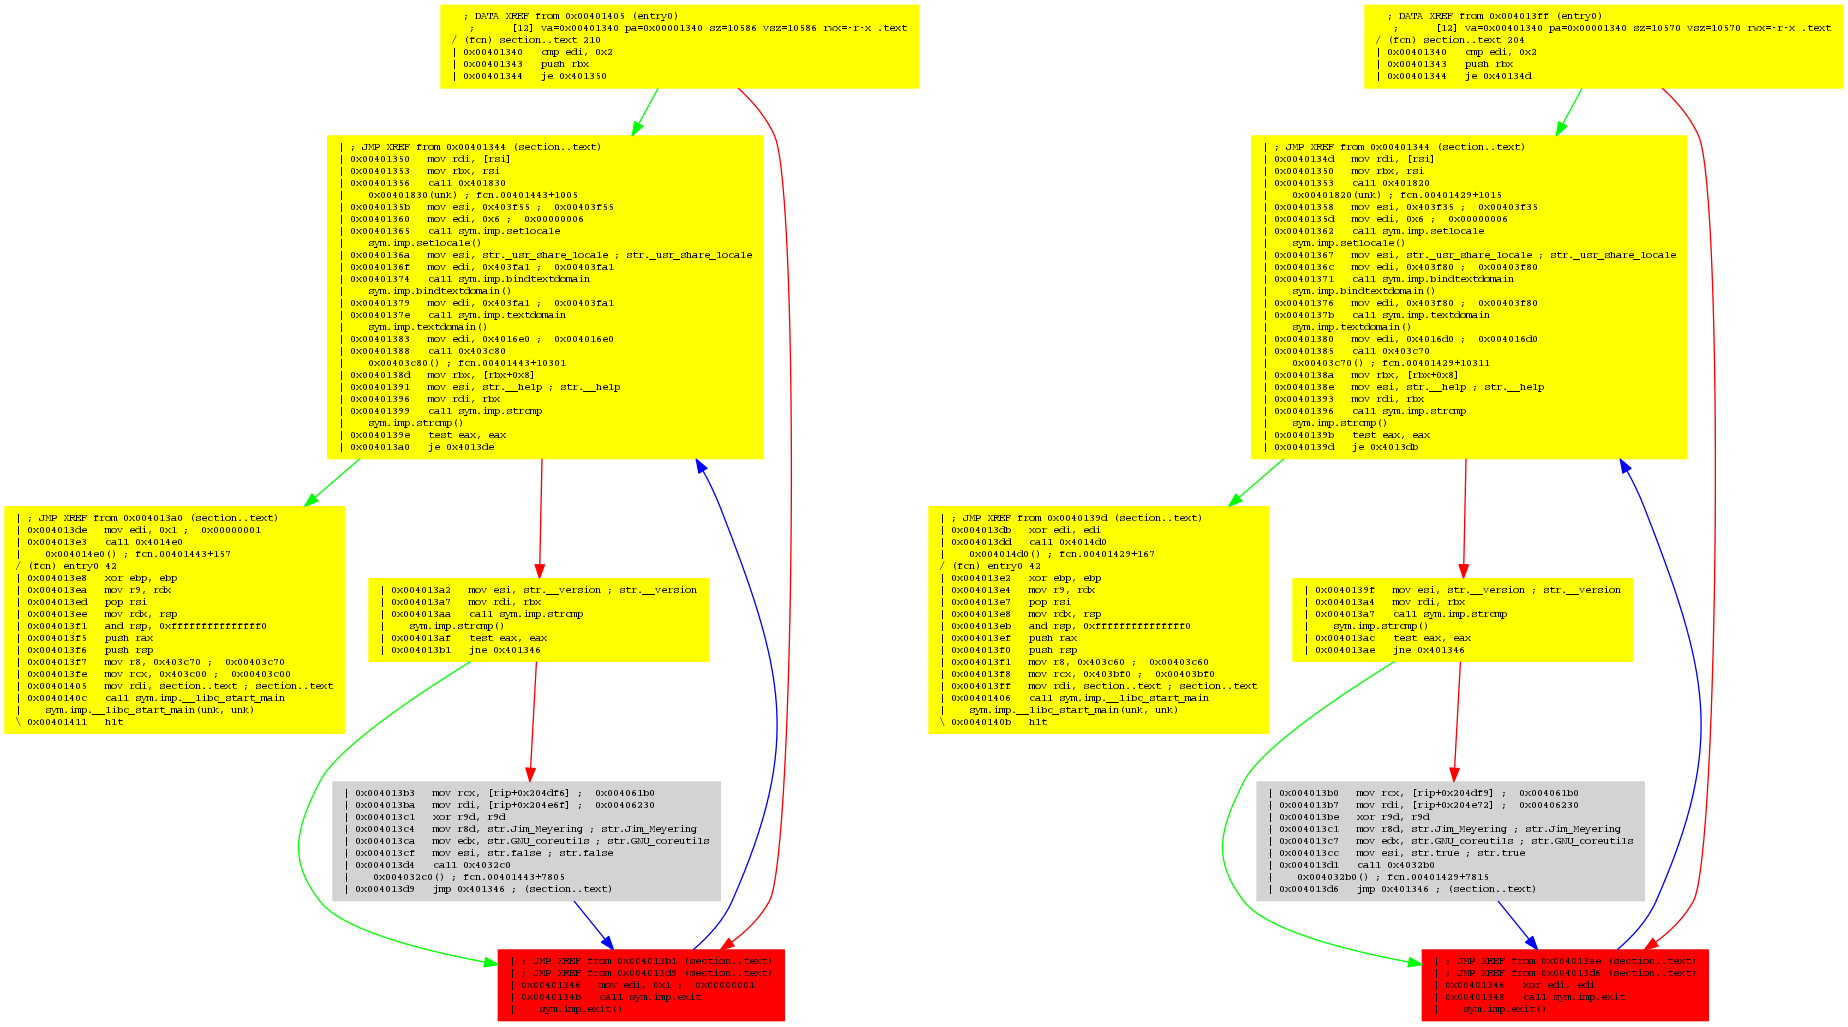
\includegraphics[width=\textwidth]{radiff2.png}
  \end{figure}
\end{frame}

\begin{frame}[fragile]
  \frametitle{Utilities}
     \begin{itemize}
        \item rax2
        \item rabin2
        \item rasm2
        \item radiff2
        \item \alert{rafind2}
        \item rahash2
        \item radare2
				\item r2pm
        \item rarun2/ragg2/ragg2-cc
      \end{itemize}
\end{frame}

\begin{frame}[fragile]
  \center\textbf{rafind2} — Advanced commandline hexadecimal editor
  \noindent\makebox[\linewidth]{\rule{\paperwidth}{0.4pt}}
  \frametitle{Utilities: rafind2}
  \begin{verbatim}$ rafind2 -X -s passwd dump.bin\end{verbatim}
  \alert{Search for the string passwd}

\end{frame}

\begin{frame}[fragile]
  \frametitle{Utilities}
     \begin{itemize}
        \item rax2
        \item rabin2
        \item rasm2
        \item radiff2
        \item rafind2
        \item \alert{rahash2}
        \item radare2
        \item rarun2
				\item r2pm
        \item rarun2/ragg2/ragg2-cc
      \end{itemize}
\end{frame}

\begin{frame}[fragile]
  \center\textbf{rahash2} — block based hashing utility
  \noindent\makebox[\linewidth]{\rule{\paperwidth}{0.4pt}}
  \frametitle{Utilities: rahash2}
  \begin{verbatim}$ rahash2 -a all binary.exe\end{verbatim}
  \alert{Display hashes of the whole file with all algos}
  \begin{verbatim}$ rahash2 -B -b 512 -a md5\end{verbatim}
  \alert{Compute md5 per block of 512}
  \begin{verbatim}$ rahash2 -B -b 512 -a entropy\end{verbatim}
  \alert{Compute md5 per block of 512}
  \begin{verbatim}$ echo -n "admin" | rahash2 -a md5 -s "\end{verbatim}
  \alert{Compute md5 of the string admin}

\end{frame}

\begin{frame}[fragile]
  \frametitle{Utilities}
     \begin{itemize}
        \item rax2
        \item rabin2
        \item rasm2
        \item radiff2
        \item rafind2
        \item rahash2
        \item \alert{radare2}
        \item rarun2
				\item r2pm
        \item rarun2/ragg2/ragg2-cc
      \end{itemize}
\end{frame}

\section{Radare2 — Command line}

\begin{frame}[fragile]
  \frametitle{1 command <—> 1 Reverse-Engineering'notion}
  Keep in mind that:
  \begin{enumerate}
  \item Every character has a meaning i.e \alert{(w = write, p = print)}
  \item Every command is a succession of character i.e \alert{pdf = p <-> print d <-> disassemble f <-> function }
  \item Every command is documented with \textbf{cmd?}, i.e \alert{pdf?},\alert{?}, \alert{???}, \alert{???}, \alert{?\$?}, \alert{?@?}
  \end{enumerate}
\end{frame}

\begin{frame}[fragile]
  \frametitle{The \# command — hashing command}
  \begin{enumerate}
  \item Open a file with radare2 \alert{radare2 file.exe}
  \item Get Usage on the command \alert{\#?} \textbf{Usage: \#algo <size> @ addr}
  \item List of all existing algorithms \alert{\#\#}
  \item SHA1 \alert{\#sha1}
  \item Hashing from the begin \alert{\#sha1 @ 0}
  \item with a hash block size corresponding to the size of the file \alert{\#sha1 \$s @ 0x0}
 \end{enumerate}
This command is same as rahash2 -a sha1 file.exe
\end{frame}

\begin{frame}[fragile]
  \frametitle{Flags}
  \begin{itemize}
  \item Flags are used to specify a name for an offset: \alert{f?}.
  \item Add a function af+ hand craft a function (requires afb+)
	\item f. name @ offset set local function label named `blah'
 \end{itemize}
 \noindent\makebox[\linewidth]{\rule{\paperwidth}{0.4pt}}
 \begin{itemize}
 \item R2 is an block-based hexadecimal editor. Change the blocksize with the ‘b’ command.
\end{itemize}
\end{frame}

\begin{frame}[fragile]
  \frametitle{The i command — information command}
  \begin{enumerate}
  \item Get Usage on the command \alert{i?}
  \item Same as \alert{rabin2}
  \item izj for displaying in json
  \item internal commands: \~, ls, \{\}, ..
 \end{enumerate}
\end{frame}

% Show Corkami PE101, ELF101,...
% Show r2 -nn on PE or an ELF
% If time explain how to parse a file format taking a PE/ELF header example (magic)
% Mention 010 editor

\begin{frame}[fragile]
  \frametitle{Radare2 — `Major' command example: pf}
  Quick Demo
\end{frame}

\begin{frame}[fragile]
  \frametitle{Radare2 - types command example}
  Quick Demo
\end{frame}

\begin{frame}[fragile]
  \frametitle{Radare2 — CLI Main commands}
  \begin{enumerate}
   \item r2 -A or r2 then aaa : Analysis
   \item s : Seek
   \item pdf : Print disassemble function
   \item af? : Analyse function
   \item ax? : Analyse XREF
   \item /? : Search
   \item ps? : Print strings
   \item C? : Comments
   \item w? : Write
 \end{enumerate}
\end{frame}

\section{Radare2 — Visual mode}
\begin{frame}[fragile]
  \frametitle{Radare2 — Visual mode Main commands}
  \begin{enumerate}
  \item V? : Visual help
  \item p/P : rotate print modes
  \item move using arrows/hjkl
  \item o : seek to
  \item e : r2configurator
  \item v : Function list
  \item \_ : HUD
  \item V : ASCII Graph
  \item 0-9 : Jump to function
  \item u : Go back
 \end{enumerate}
\end{frame}

\section{Radare2 — WebUI}
\begin{frame}[fragile]
  \frametitle{Radare2 WebUI}
  r2 -A -c=H filename
  \begin{figure}
  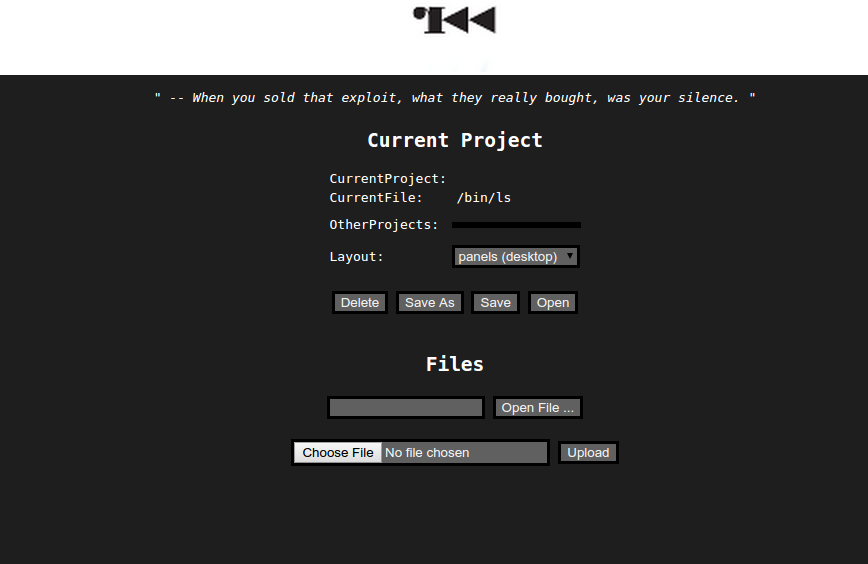
\includegraphics[width=\textwidth]{web.png}
  \end{figure}
\end{frame}

\section{Radare2 — Debugger}

\begin{frame}[fragile]
  \frametitle{Radare2 — Debugger}
  \begin{enumerate}
  \item radare2 -d
  \item Quickly switch to Visual debugger mode: Vpp
  \item OllyDBG/IDApro shortcuts friendly
 \end{enumerate}
\end{frame}

\begin{frame}[fragile]
  \frametitle{Utilities}
     \begin{itemize}
        \item rax2
        \item rabin2
        \item rasm2
        \item radiff2
        \item rafind2
        \item rahash2
        \item radare2
        \item \alert{rarun2}
				\item r2pm
        \item rarun2/ragg2/ragg2-cc
      \end{itemize}
\end{frame}

\begin{frame}[fragile]
  \frametitle{R2PM}
	\center\textbf{R2PM} — radare2 package manager
  \noindent\makebox[\linewidth]{\rule{\paperwidth}{0.4pt}}
  \begin{enumerate}
  \item r2pm -s (list all plugins)
	\item r2pm -i retdec
 \end{enumerate}
\end{frame}
\begin{frame}[fragile]
  \frametitle{Debugging}
  \begin{itemize}
	\item Native local debug (r2 -d)
	\item r2 agent (rap:// protocol)
	\item GDB remote protocol support
	\item WinDBG remote protocol support
  \end{itemize}
\end{frame}

\begin{frame}[fragile]
  \frametitle{Rarun2 \&\& Ragg2}
  \noindent\makebox[\linewidth]{\rule{\paperwidth}{0.4pt}}
  \begin{enumerate}
  \item Will be shown in Julien and Crowell'parts
 \end{enumerate}
\end{frame}

\begin{frame}[fragile]
  \frametitle{Now your turn!}
    \begin{itemize}
    \item \alert{Crackmes:} IOLI-Crackme, flare-on 2015 challenges
    \item \alert{Exploitation:} pwnablekr "bof", simple ret2libc demo, ropasaurus
    \item \alert{Malware(1/3):} Practical malware analysis samples
    \item \alert{Malware(2/3):} Any RAT samples see decoder on: https://github.com/kevthehermit/RATDecoders/
    \item \alert{Malware(3/3):} AVCaesar.lu, MalekalDB
    \item \alert{Firmware/BIOS/UEFI:} TODO
    \end{itemize}
\end{frame}

\begin{frame}[fragile]
  \frametitle{Documentation}
    \begin{itemize}
    \item \alert{Website:} http://rada.re/
    \item \alert{Blog:} http://radare.today
    \item \alert{Book:} http://radare.gitbooks.io/radare2book/content/
    \end{itemize}
\end{frame}

\begin{frame}[fragile]
  \frametitle{Scripting Capabilities}
  \center Available for a lot of programming languages
  \center\textbf{Radare2 Bindings} —
  \center\textbf{R2Pipe} —
  \noindent\makebox[\linewidth]{\rule{\paperwidth}{0.4pt}}
  \item Demo time !
\end{frame}

\section{Using r2 for exploit}
\begin{frame}{popular tools}
	\begin{itemize}
		\item gdb + peda - search memory, dereference stack/registers, debug.
		\item ida - find xrefs/calls, debug
		\item ropgadget - search for gadgets
		\item r2 can do all of this...
	\end{itemize}
\end{frame}

\begin{frame}{getting binary info}
	\begin{itemize}
		\item "checksec" - get info : pie, stack canaries, nx
		\item find strings - find references to calls, etc.
		\item find writable/executable sections
	\end{itemize}
\end{frame}

\begin{frame}{getting binary info}
	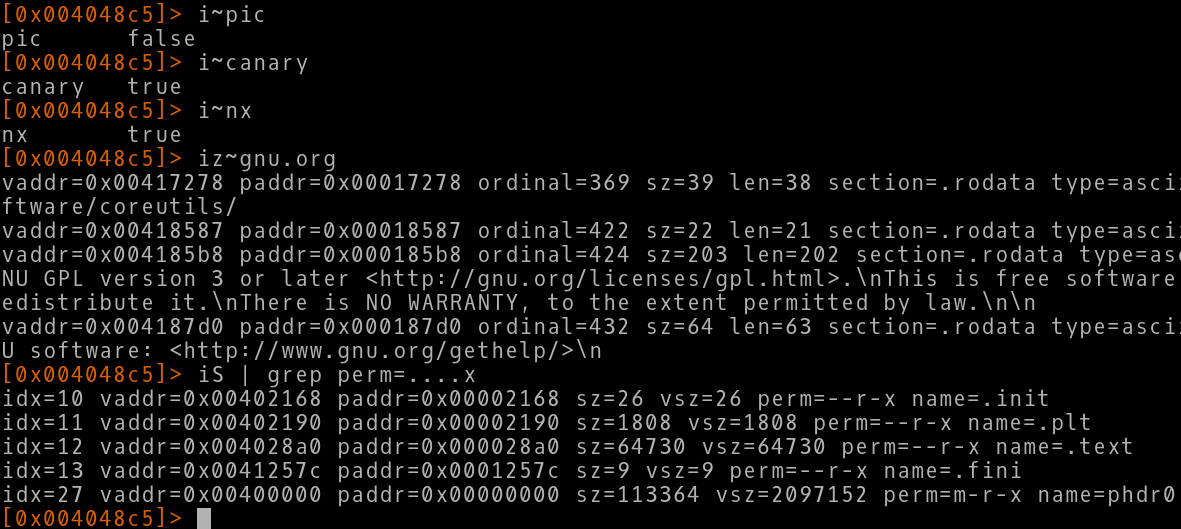
\includegraphics[width=\textwidth]{crimages/bin-info.png}
\end{frame}

\begin{frame}{"telescoping" register}
	\begin{columns}
		\begin{column}{.3\textwidth}
			\begin{itemize}
				\item "telescoping" registers
				\item "telescoping" stack references
				\item we lose our analysis capabilities on gdb
			\end{itemize}
		\end{column}
		\begin{column}{.7\textwidth}
			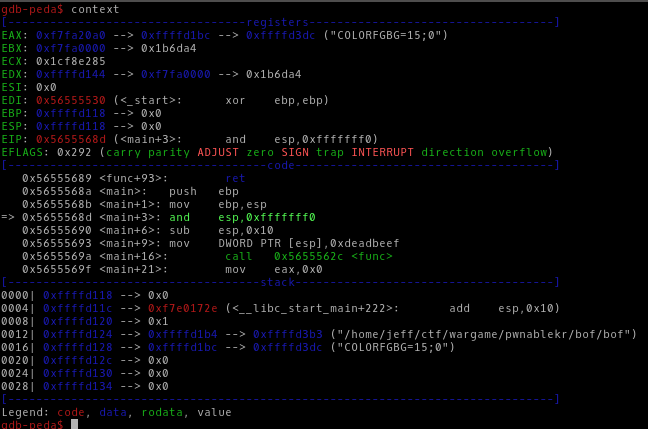
\includegraphics[width=\textwidth]{crimages/peda_context.png}
		\end{column}
	\end{columns}
\end{frame}

\begin{frame}{"telescoping" register}
	\begin{columns}
		\begin{column}{.3\textwidth}
			\begin{itemize}
				\item we can do the same thing with r2
				\item display references to code/ascii/etc. from registers/stack
				\item quite useful for dynamic analysis.
				\item keep flags, symbols, etc.
				\item drr (registers) pxr N @ esp/rsp (stack)
			\end{itemize}
		\end{column}
		\begin{column}{.7\textwidth}
			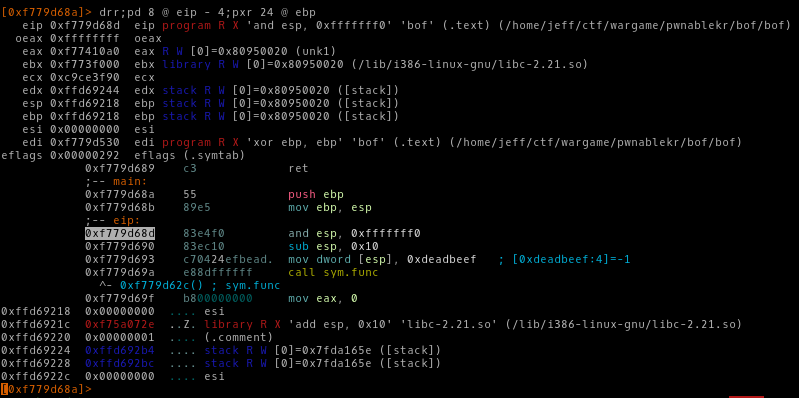
\includegraphics[width=\textwidth]{crimages/r2_context1.png}
		\end{column}
	\end{columns}
\end{frame}

\begin{frame}{knowing context is useful}
	\begin{itemize}
		\item does your register point to a string you control?
		\item what's in the stack?
		\item keep flags, symbols, etc.
		\item use from within visual mode `e dbg.slow = true`
	\end{itemize}
\end{frame}

\begin{frame}{pattern generate}
	\begin{itemize}
		\item DeBruijn patterns.
		\item made famous by metasploit pattern\_create.rb
		\item cyclic patterns, find offset in string.
		\item Where's our faked struct/string/etc. being referenced?
		\item Where did we crash?
		\item ragg2 -P -r or woD to write
		\item ragg2 -q or woO to find your offset.
	\end{itemize}
\end{frame}

\begin{frame}{debug 'profiles'}
	\begin{itemize}
		\item r2 -de dbg.profile=file.rr2 exec.elf
		\item set custom arguments, redirect stdin/out to files/sockets
		\item useful for reproducing environments
	\end{itemize}
\end{frame}

\begin{frame}{context + patterns}
	\begin{itemize}
		\item bof from pwnable.kr
		\item super simple challenge, overflow a buffer
		\item offset at a certain place must be.
		\item let's use rarun2 + references + patterns!
	\end{itemize}
\end{frame}

\begin{frame}{context + patterns}
	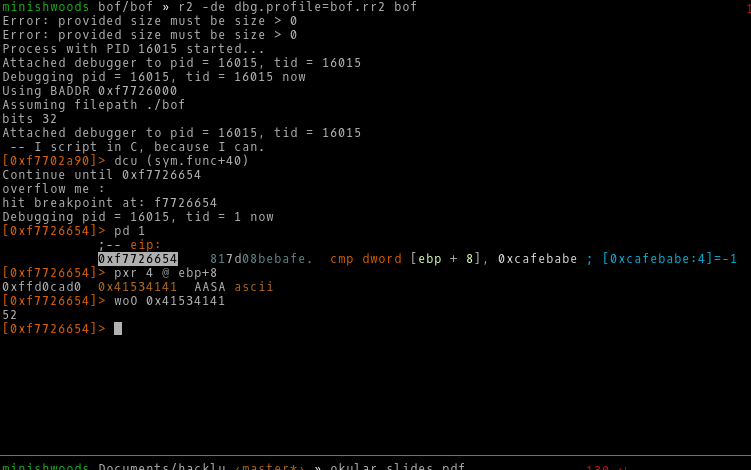
\includegraphics[width=\textwidth]{crimages/bof1.png}
	\begin{itemize}
		\item write your own expl ;)
	\end{itemize}
\end{frame}


\begin{frame}{shellcoding}
	\begin{itemize}
		\item ragg2 isn't just for generating patterns
		\item front-end for generating shellcodes
		\item still up to you to ensure null-free, etc.
	\end{itemize}
\end{frame}

\begin{frame}{shellcoding}
	\begin{itemize}
		\item relocatable
		\item testable (compile directly into elf)
		\item call arbitrary syscalls easily!
		\item x86, amd64, arm, windows, mac, linux, ios
	\end{itemize}
\end{frame}

\begin{frame}{shellcoding}
	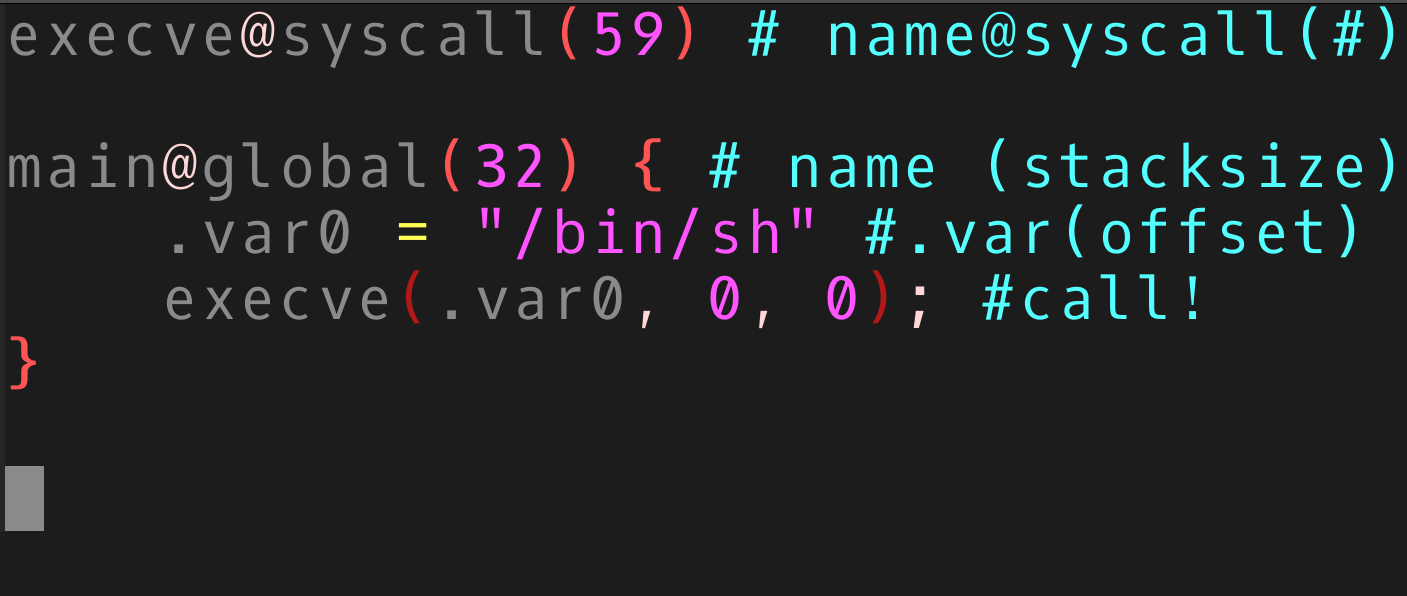
\includegraphics[width=\textwidth]{crimages/shellcode.png}
	\begin{itemize}
		\item ragg2 file.r -s to show the emmitted asm.
	\end{itemize}
\end{frame}

\begin{frame}{code reuse}
	\begin{itemize}
		\item return to libc
		\item rop
		\item r2 can make this easy
	\end{itemize}
\end{frame}

\begin{frame}{code reuse}
	\begin{itemize}
		\item magic shell-spawning gadget
		\item thanks dragon sector for making this well-known
		\item exists in amd64 glibc, libruby, and more...
		\item let's find it with r2
	\end{itemize}
\end{frame}

\begin{frame}{code reuse}
	\begin{itemize}
		\item demo
		\item r2 -A /path/to/libc
		\item axt sym.execve
		\item through xrefs, find it.
		\item simple demo program on vm does 1 call of your base10 input address
	\end{itemize}
\end{frame}

\begin{frame}{rop}
	\begin{itemize}
		\item can't always use this magic gadget
		\item rsi must point to something argv-like
		\item sometimes need to find some odd bespoke gadget!
		\item r2 can dump gadgets
		\item regular expression search
		\item dump to json, write your own tool via r2pipe.
	\end{itemize}
\end{frame}

\begin{frame}{stack layout}
	\begin{itemize}
			\item when you "ret"
			\item ebp is increased by 4, jump to new\_ebp - 4
			\item add esp,4
			\item jmp dword ptr [esp-4]
	\end{itemize}
\end{frame}

\begin{frame}{searching for gadgets}
	\begin{itemize}
			\item sequence of instructions followed by "end/stop" gadget
			\item (arbitrary instructions) - ret/call/jmp/etc...
			\item finding the right ones is hard, r2 has regexp support
			\item we can set variable filters.
	\end{itemize}
\end{frame}

\begin{frame}{demo time}
	\begin{itemize}
			\item super basic rop expl.
			\item combine finding sections, patterns, rop search.
			\item r2 makes this easy
	\end{itemize}
\end{frame}

\begin{frame}{searching for gadgets}
	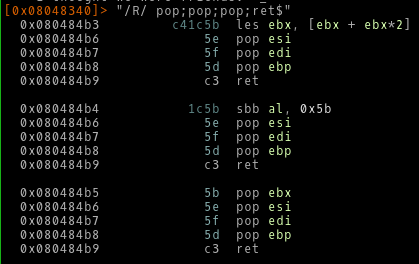
\includegraphics[width=\textwidth]{crimages/poppopret.png}
\end{frame}

\section{Debugging}
\begin{frame}[fragile]
  \frametitle{GDB protocol}
  \center Just run gdbserver somewhere
  \center and connect r2 to it:
  \center r2 -D gdb -d /bin/ls gdb://99.44.23.50:4589
\end{frame}

\begin{frame}[fragile]
  \frametitle{GDB protocol + Wine}
  \center Winedbg allows to run windows command
  \center using the gdbserver too:
  \center winedbg --gdb --no-start malware.exe
  \center r2 -a x86 -b 32 -D gdb -d malware.exe gdb://localhost:44840
\end{frame}

\begin{frame}[fragile]
  \frametitle{WinDBG}
\ifxetex
  \center r2 allows to connect WinDBG/KD
\else
  \center r2 allows to connect WinDBG/KD \footfullcite{r2windbg}
\fi
  \center For example, to debug windows kernel via the serial port:
  \center bcdedit /debug on
  \center bcdedit /dbgsettings serial debugport:1 baudrate:115200
  \center then connect r2:
  \center r2 -a x86 -b 32 -D wind windbg:///tmp/windbg.pipe
  \center For now, connecting to the QEMU and VirtualBox are tested
% More information here https://github.com/radare/radare2/blob/master/doc/windbg
\end{frame}

\begin{frame}[fragile]
  \frametitle{Debugging OMAP BootRom}
  \center Just run it in the modified qemu https://github.com/XVilka/qemu
  \center ./configure --target-list=arm-softmmu ; make ; sudo make install
  \center qemu-system-arm -M milestone -m 256 -L . -bios bootrom.bin -mtdblock	mbmloader-1.raw -d in\_asm,cpu,exec -nographic -s -S
  \center r2 -D gdb -b arm gdb://localhost:9999
  \center Same approach could be used for any customized hardware
\end{frame}

% show demo here - demos/demo1_arm_boot

\begin{frame}[fragile]
  \frametitle{GDB protocol + Wine}
  \center Winedbg allows to run windows command
  \center using the gdbserver too:
  \center winedbg --gdb --no-start malware.exe
  \center r2 -a x86 -b 32 -D gdb -d malware.exe gdb://localhost:44840
\end{frame}

\section{Firmware analysis}
\begin{frame}[fragile]
  \frametitle{UEFI analysis}
  \begin{itemize}
    \item Dump the image using flashrom or hardware
\ifxetex
	\item Unpack the image using UEFITool
\else
	\item Unpack the image using UEFITool \footfullcite{uefitool}
\fi
	\item Open the selected PE or TE file using r2
  \end{itemize}
\end{frame}

% show demo here - demos/demo3_x86_uefi
% Before starting, you can mention, that we need full UEFI image from the SPI flash
% We'll use the ready dump, but at home, they can run 'flashrom' tool on their
% computers, to dump the image, using the 'internal' programmer, or any external one.
% After the modification with r2 and UEFITool they can flash it back using the same
% programmer and flashrom. Also please say, that this can brick their computers,
% so better not to start without backup (external programmer) or if they
% are adventurous enough.
% 1. download UEFITool here https://github.com/LongSoft/UEFITool
% 2. run 'qmake' in its sources
% 3. run 'make' in its sources
% 4. run resulting 'UEFITool' binary, choose 'Open image' -> hp_image.bin
% 5. show the tree, find some example e.g. 'PchInit' module, choose 'Extract body'
% and save it to the file, 'PchInit.efi' (tell that those EFI files are simple PE)
% 6. Open that file in the radare2: 'r2 -w PchInit.efi'
% 7. Patch some commands/data in it, write, exit r2
% 8. Open UEFITool again, choose 'Replace body', open that changed 'PchInit.efi'
% 9. Save the resulting image into the new file, e.g. hp_image_mod.bin

\begin{frame}[fragile]
  \frametitle{Old legacy BIOS analysis}
  % This shows the example of talking to the SMBus
  \begin{itemize}
\ifxetex
	\item Load the whole image or unpack it using bios\_extract
\else
    \item Load the whole image or unpack it using bios\_extract \footfullcite{bios-extract}
\fi
	\item Open it using the correct segment and offset
	\item r2 load the whole BIOS image automatically
	\item r2 asrock\_p4i65g.bin
	\item >. asrock\_p4i65g.r2
  \end{itemize}
\end{frame}

\begin{frame}[fragile]
  \frametitle{The t command — types management}
  \begin{enumerate}
\ifxetex
  \item Get Usage on the command \alert{t?}
\else
  \item Get Usage on the command \alert{t?} \footfullcite{r2types}
\fi
  \item \alert{to} to load the types from the C header file
  \item \alert{tl} link type to the memory, \alert{tf} shows it like the pf
  \item add \alert{j} to get the output in the json format
 \end{enumerate}
\end{frame}

% This demo is in demos/demo3_x86_legacy
% 1. Open 'r2 -a x86 asrock_p4i65g.bin'  - it should recognize legacy BIOS format automatically
% (x86, 16bit)
% 2.'[f000:fff0]> . asrock_p4i65g.r2' - add some comments and functions in the loaded fresh file
% 3.'[f000:4736]> to asrock_p4i65g.h'
% 4.'[f000:4736]> t' - list all loaded types
% 5.'[f000:4736]> s SIO_Init' - go to the SIO_Init() function address
% 6.'[f000:5c93]> Vp' - show the code, tell that lines mov si, 0x5c50 ; lodsw ax, word cs:[si] is
% actually reading some data, after some background research we've found this is a table of the
% SuperIO registers, so we can apply structure here, to see the values
% 7.'[f000:5c93]> tl SIO_reg_mask 0xf000:0x5c50' - link the structure 'SIO_reg_mask' to the 0xf000:0xfc50 address
% 8.'[f000:5c93]> tf 0xf000:0x5c50' - shows the values (be careful, there is a bug, don't attract
% attention that it shows dwords instead of chars (should be char) from the structure description.

% Additional information here http://radare.today/types/


% show demo here - demos/demo3_x86_legacy
% download bios_extract here http://www.coreboot.org/Bios_extract
\begin{frame}[fragile]
  \frametitle{Embedded controller - 8051}
  \center Lets start from the static analysis
  \center r2 -a 8051 ite\_it8502.rom
  \center >. ite\_it8502.r2
\end{frame}

% show demo here - demos/demo5_it8502e

\begin{frame}[fragile]
  \frametitle{Embedded controller - 8051 - ESIL VM}
\ifxetex
  \center Lets start from the static analysis
\else
  \center Lets start from the static analysis \footfullcite{r2esiltv}
\fi
  \center r2 -a 8051 ite\_it8502.rom
  \center . ite\_it8502.r2
  \center run `e io.cache=true' to use the cache for write operations
  \center run `aei' command to init ESIL VM
  \center run `aeim' command to init ESIL VM stack
  \center run `aeip' command to start from the current offset
  \center run `aecu [addr]' to emulate until the [addr] is reached
\end{frame}
% show demo here
% Reference to the example from here? http://radare.tv/a/44

\begin{frame}[fragile]
  \frametitle{Embedded controller - 8051 - ESIL2REIL}
  \center Lets start again from the same place
  \center r2 -a 8051 ite\_it8502.rom
  \center . ite\_it8502.r2
  \center run `pae 36' to show the esil expression of the `set\_SMBus\_frequency'
  \center run `aetr \`{}pae 36\`' to convert the previous esil output to REIL
  \center store this to some file and use the `openreil' utility to SMT it
\end{frame}
% this is:
% aetr `pae 36`
% reference to the https://github.com/Cr4sh/openreil
% what about some demo for that?

\begin{frame}[fragile]
  \frametitle{Documentation}
    \begin{itemize}
    \item \alert{Website:} http://rada.re/
    \item \alert{Blog:} http://radare.today
    \item \alert{Book:} http://maijin.gitbooks.io/radare2book/content/
    \end{itemize}
\end{frame}

\ifxetex
\else
\section{References}
\begin{frame}[allowframebreaks]
	\frametitle{A lot of them}
	\printbibliography
\end{frame}
\fi

\end{document}
